%%
%% This is file `sample-sigconf.tex',
%% generated with the docstrip utility.
%%
%% The original source files were:
%%
%% samples.dtx  (with options: `sigconf')
%% 
%% IMPORTANT NOTICE:
%% 
%% For the copyright see the source file.
%% 
%% Any modified versions of this file must be renamed
%% with new filenames distinct from sample-sigconf.tex.
%% 
%% For distribution of the original source see the terms
%% for copying and modification in the file samples.dtx.
%% 
%% This generated file may be distributed as long as the
%% original source files, as listed above, are part of the
%% same distribution. (The sources need not necessarily be
%% in the same archive or directory.)
%%
%% The first command in your LaTeX source must be the \documentclass command.
\documentclass[sigconf]{acmart}

\usepackage{listings}
\lstset{
	language=Java,
	breaklines,
}
\graphicspath{{images/}}
\DeclareGraphicsExtensions{.pdf,.png,.jpg}


%%
%% \BibTeX command to typeset BibTeX logo in the docs
\AtBeginDocument{%
  \providecommand\BibTeX{{%
    \normalfont B\kern-0.5em{\scshape i\kern-0.25em b}\kern-0.8em\TeX}}}

%% Rights management information.  This information is sent to you
%% when you complete the rights form.  These commands have SAMPLE
%% values in them; it is your responsibility as an author to replace
%% the commands and values with those provided to you when you
%% complete the rights form.
%\setcopyright{acmcopyright}
%\copyrightyear{2020}
%\acmYear{2020}
%\acmDOI{10.1145/1122445.1122456}

%% These commands are for a PROCEEDINGS abstract or paper.
%\acmConference[I3D’19]{ACM Symposium on Parallelism in Algorithms and Architectures}{July 14--17, 2020}{Philadelphia, PA, USA}
%\acmBooktitle{Woodstock '18: ACM Symposium on Neural Gaze Detection,
 % June 03--05, 2018, Woodstock, NY}
%\acmPrice{15.00}
%\acmISBN{978-1-4503-XXXX-X/18/06}


%%
%% Submission ID.
%% Use this when submitting an article to a sponsored event. You'll
%% receive a unique submission ID from the organizers
%% of the event, and this ID should be used as the parameter to this command.
%%\acmSubmissionID{123-A56-BU3}

%%
%% The majority of ACM publications use numbered citations and
%% references.  The command \citestyle{authoryear} switches to the
%% "author year" style.
%%
%% If you are preparing content for an event
%% sponsored by ACM SIGGRAPH, you must use the "author year" style of
%% citations and references.
%% Uncommenting
%% the next command will enable that style.
%%\citestyle{acmauthoryear}

%%
%% end of the preamble, start of the body of the document source.
\begin{document}

%%
%% The "title" command has an optional parameter,
%% allowing the author to define a "short title" to be used in page headers.
\title{Application of concatenable queue for parallel computational geometry algorithms}

%%
%% The "author" command and its associated commands are used to define
%% the authors and their affiliations.
%% Of note is the shared affiliation of the first two authors, and the
%% "authornote" and "authornotemark" commands
%% used to denote shared contribution to the research.

%\author{Vasyl Tereshchenko}
%\authornote{Both authors contributed equally to this research.}
%\email{vtereshch@gmail.com}
%\orcid{0000-0002-0139-6049}
%\author{Semen Chudakov}
%\authornotemark[1]
%\email{semen.chudakov7@gmail.com}
%\affiliation{%
%  \institution{Taras Shevchenko National University of Kyiv}
%  \streetaddress{P.O. Box 01601}
%  \city{Kyiv}
%  \state{}
%  \postcode{}
%}

%\author{Lars Th{\o}rv{\"a}ld}
%\affiliation{%
%  \institution{The Th{\o}rv{\"a}ld Group}
%  \streetaddress{1 Th{\o}rv{\"a}ld Circle}
%  \city{Hekla}
%  \country{Iceland}}
%\email{larst@affiliation.org}

%\author{Valerie B\'eranger}
%\affiliation{%
%  \institution{Inria Paris-Rocquencourt}
%  \city{Rocquencourt}
%  \country{France}
%}

%\author{Aparna Patel}
%\affiliation{%
% \institution{Rajiv Gandhi University}
% \streetaddress{Rono-Hills}
% \city{Doimukh}
% \state{Arunachal Pradesh}
% \country{India}}

%\author{Huifen Chan}
%\affiliation{%
%  \institution{Tsinghua University}
%  \streetaddress{30 Shuangqing Rd}
%  \city{Haidian Qu}
%  \state{Beijing Shi}
%  \country{China}}

%\author{Charles Palmer}
%\affiliation{%
%  \institution{Palmer Research Laboratories}
%  \streetaddress{8600 Datapoint Drive}
%  \city{San Antonio}
%  \state{Texas}
%  \postcode{78229}}
%\email{cpalmer@prl.com}

%\author{John Smith}
%\affiliation{\institution{The Th{\o}rv{\"a}ld Group}}
%\email{jsmith@affiliation.org}

%\author{Julius P. Kumquat}
%\affiliation{\institution{The Kumquat Consortium}}
%\email{jpkumquat@consortium.net}

%%
%% By default, the full list of authors will be used in the page
%% headers. Often, this list is too long, and will overlap
%% other information printed in the page headers. This command allows
%% the author to define a more concise list
%% of authors' names for this purpose.
%\renewcommand{\shortauthors}{Tereshchenko and Chudakov}

%%
%% The abstract is a short summary of the work to be presented in the
%% article.
\begin{abstract}
	The paper is devoted to the development and  of an efficient algorithmic model for solving a set of interrelated computational geometry problems. To do this, a unified algorithmic environment with unified data structures is created, which allows to implement complex use cases efficiently with respect to computational resources. We build the environment on the basis of the ``divide and conquer'' strategy. 
	Once a convex hull is key to a set of computational geometry problems, we offer a concatenable queue data structure to maintain it. The data structure is implemented in a form of a binary tree. This allows to perform operations needed in algorithm for a set of problems in $O(\log n)$ time. Furthermore we offer a way to execute the algorithms both sequentially and in parallel.
	In the future the algorithmic environment can be improved to support other computational models with similar properties for solving problems. As an example, the Voronoi diagram or the Delaunay triangulation can be considered.
\end{abstract}

%%
%% The code below is generated by the tool at http://dl.acm.org/ccs.cfm.
%% Please copy and paste the code instead of the example below.
%%

%%
%% Keywords. The author(s) should pick words that accurately describe
%% the work being presented. Separate the keywords with commas.
\keywords{unified data structure, parallel algorithms, interrelated problems set, unified algorithmic environment, concatenable queue}

%% A "teaser" image appears between the author and affiliation
%% information and the body of the document, and typically spans the
%% page.
%%
%% This command processes the author and affiliation and title
%% information and builds the first part of the formatted document.
\maketitle

\section{Introduction}
\label{sec:introduction}

	Nowadays, advanced computer simulations and visualizing of complex scientific researches as well as large scale technical projects requires to simultaneously solve a set of problems. The core of this set are problems of computational geometry and computer graphics. To solve such problems it is needed to create suitable algorithmic frameworks, that would yield accurate results in real time. Existing methods (iLastic \cite{ilastik}, IMARIS \cite{imaris}, ImageJ \cite{imagej}), that are based on a set of algorithms implementations organized in a package does not result in desirable efficiency and accuracy. It is worth noting, that there are a lot of parallel algorithms designed to solve specifically certain computational geometry problems such as in \cite{aggarwal,atallah,cole,amato,chen,berkman,goodman,akl,jaja,leeuwen,reif}. Every such algorithm requires its own computational resources and is executed independently from others. In such case some identical steps, such as preprocessing and building data structures, are performed several times. 

	Therefore, an important objective in developing the algorithmic models is to create a universal tool, which would have means to efficiently solve a set of problems. This tool should also execute identical steps of the algorithms once and be able to represent results of those steps in a form of the unified data structures. In \cite{tereshchenko} the notion of a unified algorithmic environment is introduced, which is based on the ``divide-and-conquer'' principle and takes into account the aforementioned features of the algorithms. In particular, the preprocessing and splitting the initial set of data to form the recursion tree is common for all problems and is executed only once. During the merge stage intermediate results are maintained in a weighted concatenable queue. This model does not repeat computations and the intermediate results are highly reused during the algorithms, which yields good performance.

	In this article we first describe how the convex hull algorithm for a static set of points is decomposed into separate stages and incorporated into our unified algorithmic environment model (UAEM). Then we provide detailed explanation on how the concatenable queue which is used in the algorithm is implemented. Finally we make complexity analysis for the algorithm and evaluate its performance.

\section{Unified algorithmic environment}
\label{sec:unified-algorithmic-environment}
\subsection{Algorithms stages}


% //////////////////////////////////////////////////////////////////////////////////////////////////////////////////////////
% ----------------------------------------------- PROBLEM STATEMENT --------------------------------------------------------
% //////////////////////////////////////////////////////////////////////////////////////////////////////////////////////////


	In this section we describe the principle of how we decompose each algorithm into distinct parts. This partition is then used to avoid repeating the computations in the algorithmic environment. The principle will be show on a convex hull algorithm which is similar to the one describe in \cite{overmars} but operates on a static set of points.

	The notion of a convex hull is simple. For a set of points $S$ in a $k$-dimensional space it is a smallest convex set, that comprise $S$. In practice to solve such problem, means to find a subset in $S$, which can be a "skeleton" for the convex hull.


% //////////////////////////////////////////////////////////////////////////////////////////////////////////////////////////
% ----------------------------------------------- PREPROCESSING ------------------------------------------------------------
% //////////////////////////////////////////////////////////////////////////////////////////////////////////////////////////

		In the preprocessing stage, the "inner" points, which lie on a horizontal or vertical line, are removed from the set. Formally, the removal criterion is formulated as follows. For $a = (x_a, y_a)$ we denote $x(a)=x_a$, $y(a)=y_a$. Let points $a_1, a_2, ..., a_k$ lie on one horizontal line and $x(a_1) < x(a_2) <... <x (a_k) $. Then, by the criterion, the points $a_2, a_3, ..., a_{k-1}$ must be removed. Similarly for the vertical case.
		
		Consider an algorithm that, in a sorted array, for each group of identical elements, deletes all but the first and the last (if the repetition is more than two). The idea behind the algorithm is to use two pointers to delete repetitions by overwriting their place with other non-repeating element. In this way, additional memory usage can be reduced to a constant value. The algorithm makes one pass through the array. At each step, a constant amount of work is performed to decide whether to delete the current item. Given this, the complexity of the above algorithm is $O(n)$.
		
		To perform the preprocessing described above, it is needed to:
		
		\begin{enumerate}
			\item
			Sort points by $y$ (if $y$ coordinates are equal, the $x$ coordinates are compared).
			\item
			Delete repetitions by $y$ coordinate using the described algorithm.
			\item
			Sort points by $x$ (if $x$ coordinates are equal, the $y$ coordinates are compared).
			\item
			Delete repetitions by $x$ coordinate using the described algorithm.
		\end{enumerate}
	
		In the result we get a set of points for which we can apply the recursive convex hull algorithm.
		
% //////////////////////////////////////////////////////////////////////////////////////////////////////////////////////////
% ----------------------------------------------- SPLIT ------------------------------------------------------------
% //////////////////////////////////////////////////////////////////////////////////////////////////////////////////////////

		
		At the stage of splitting the initial problem, the current set of points is divided into left and right parts of equal size. Since a list is used to store the points, this operations can be completed in $O(1)$ using the formula below:
		
		\begin{equation}
			M_{i,j}=\frac{i+j}{2}
		\end{equation}
		The recursion stops when there are no more than $3$ points in the set.
		
		For the base case, the set of points can have $2$ or $3$ elements. In the first case the highest of two points forms the upper part of the hull, and the lower - the lower part.
		To consider the base case of $3$ points, we introduce an additional notion of the tangent slope given by two points on the plane. For arbitrary points $a_1, a_2$ such that $x(a_1)<x(a_2)$ slope is denoted as $\lambda$:
		
		\begin{equation}
			\lambda(a_1, a_2)=\frac{y(a_2)-y(a_1)}{x(a_2)-x(a_1)}
		\end{equation}
		According to this definition, the possible cases for points $a_1,a_2,a_3$ are given in Table \ref{table:3points}:
		
		\begin{table}[htbp]
			\caption{3-points base cases}
			\label{table:3points}
			\begin{center}
				\begin{tabular}{|c|c|c|c|}
					\hline
					\textbf{$\lambda(a_1, a_2) > \lambda(a_2, a_3)$} & \textbf{$y(a_1) < y(a_2)$} & upper part & lower part\\
					\hline
					false & false & $a_1, a_3$ & $a_2$ \\
					\hline
					false & true & $a_1, a_3$ & $a_2$ \\
					\hline
					true & false & $a_2, a_3$ & $a_1$ \\
					\hline
					true & true & $a_1, a_2$ & $a_3$ \\
					\hline
				\end{tabular} 
			\end{center}
		\end{table} 
	
% //////////////////////////////////////////////////////////////////////////////////////////////////////////////////////////
% --------------------------------   THE MERGE STEP ------------------------------------------------------------------------
% //////////////////////////////////////////////////////////////////////////////////////////////////////////////////////////

		\cite{overmars} provides an algorithm for merging two convex hulls. The essence of the algorithm is to maintain the hull with the help of two concatenated queues. The hull is divided into two parts. In this article, the separation occurs from top to bottom. Then, using the two-pointer technique and the cases described in \cite{overmars}, the proper tangent line is searched. It remains to split the two queues at the 2 found vertices that form the tangent and to merge the remaining parts. An example of performing such a procedure is shown in Fig. \ref{fig:ch_union}.
		
		\begin{figure}[htbp]
			\centerline{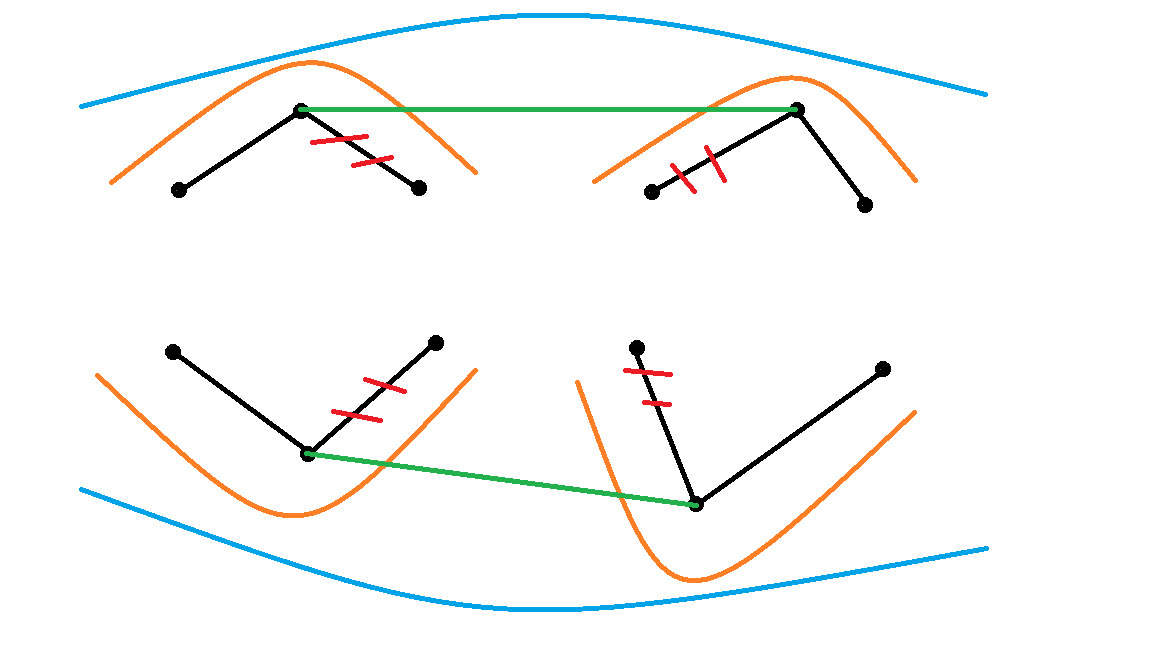
\includegraphics[width=0.4\textwidth, height=0.2\textheight]{ch_union}}
			\caption{Merging step of two hulls}
			\label{fig:ch_union}
		\end{figure}
		
		It remains to consider the corner cases that arise when performing the merging. The first of these cases is related to the ambiguity of the position of the utmost points in the described representation of the convex hull. The leftmost point of the left hull and the rightmost point of the right hull must belong to the upper parts of the view before finding the tangent line, because otherwise such tangent may be found incorrectly. An example of such incorrect search is given in Fig. \ref{fig:incorect_search}.
		
		\begin{figure}[htbp]
			\centerline{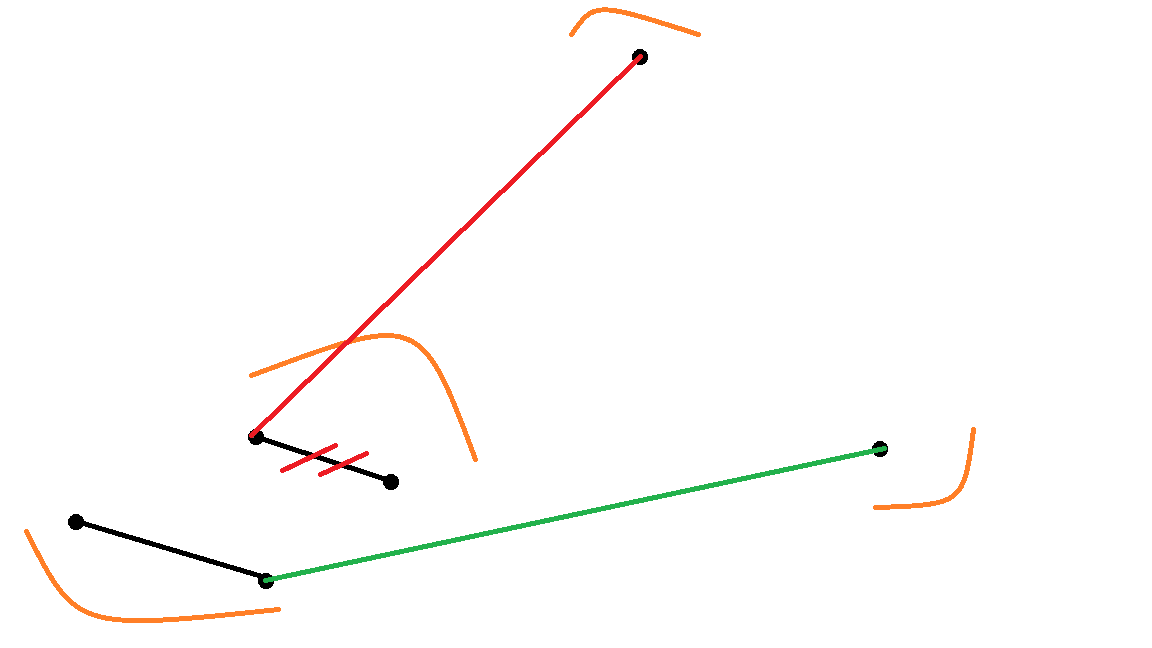
\includegraphics[width=0.4\textwidth, height=0.2\textheight]{incorect_search}}
			\caption{Example of an incorrect position of the utmost left in the left sub-hull}
			\label{fig:incorect_search}
		\end{figure}
		
		To avoid such a situation, it is necessary to move the indicated points from their upper parts before merging the sub-hulls. For the rightmost point of the left hull and the leftmost point of the right hull we have the following cases. Similarly to the previous argument, they must be transferred to the upper parts of the hulls. And after merging these points must be transferred to the lower parts of the hull, if they do not belong to the created upper part of the final hull. Otherwise, the formed hull may be incorrect. An example of such case is shown in Fig. \ref{fig:incorect_edge_points}.
		
		
		\begin{figure}[htbp]
			\centerline{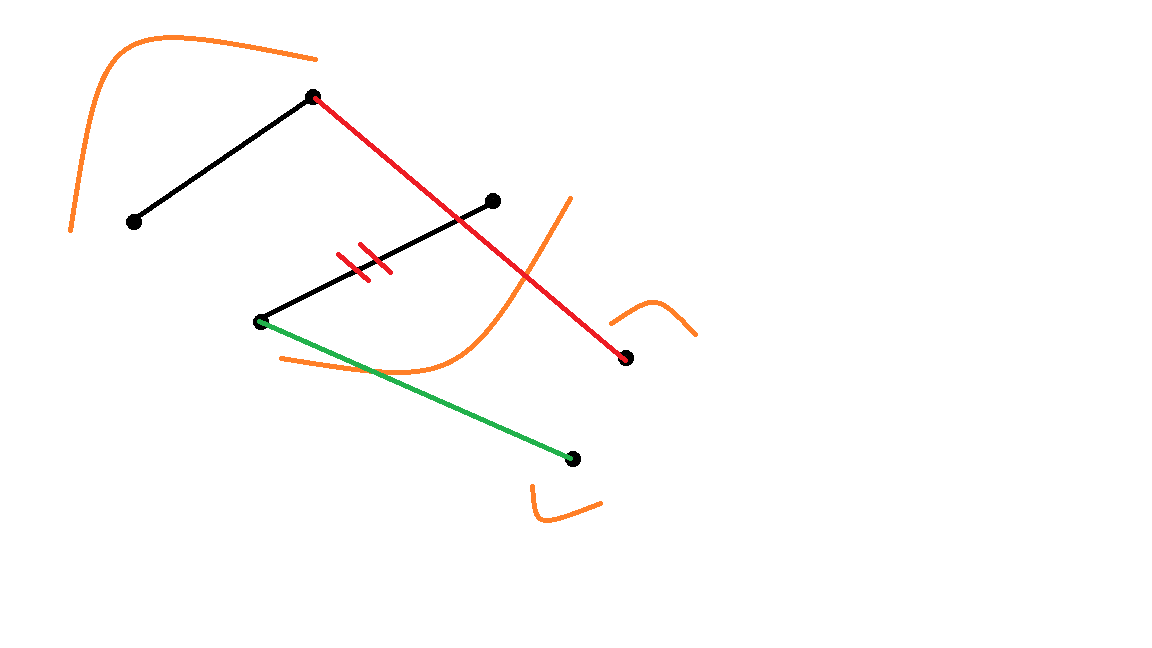
\includegraphics[width=0.4\textwidth, height=0.2\textheight]{incorect_edge_points}}
			\caption{Example of a convex hull for a wrong position of the utmost left points of the left sub-hull}
			\label{fig:incorect_edge_points}
		\end{figure}
		
		After combining the parts of the convex hulls, another corner case might take place. The search for the tangent for the upper parts of the hulls does not take into account the position of the lower parts and vice versa. As a result, the upper and lower parts of the final hull may not form a coherent structure. An example of such a situation is shown in Fig. \ref{fig:incorect_lower_subhull}.
		
		\begin{figure}[htbp]
			\centerline{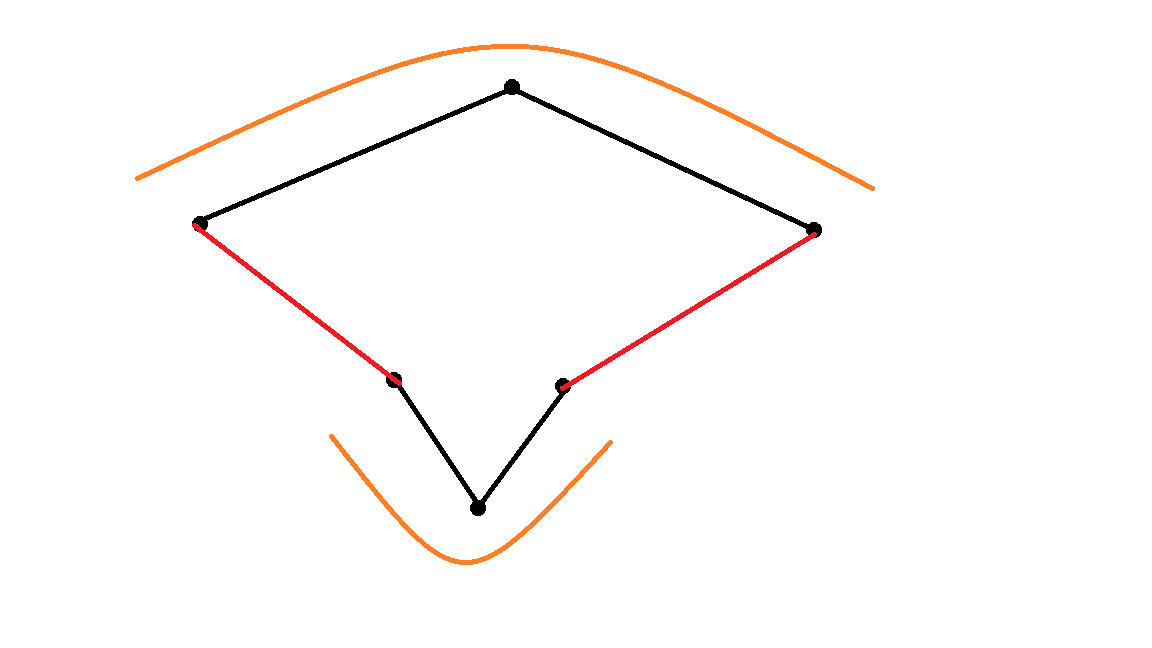
\includegraphics[width=0.4\textwidth, height=0.2\textheight]{incorect_lower_subhull}}
			\caption{An example of a non-integral hull after merging along the reference lines}
			\label{fig:incorect_lower_subhull}
		\end{figure}
		
		To avoid such a situation, it is necessary to perform the step of cutting off the redundant parts of the formed lower sub-hull. Then searching for the left and right pivoting vertices in the concatenable queue is performed. After that, the queue is splits over the found vertices.
		Fig. \ref{fig:correct_convex_hull} shows correct convex hull.
		
		\begin{figure}[htbp]
			\centerline{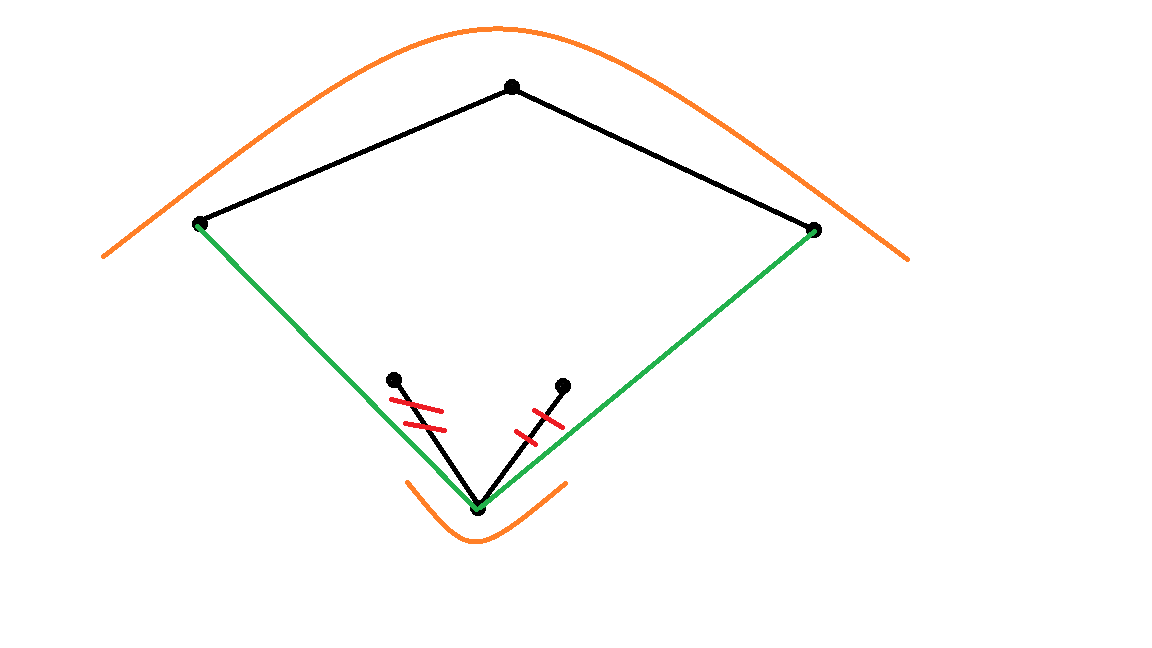
\includegraphics[width=0.4\textwidth, height=0.2\textheight]{correct_convex_hull}}
			\caption{Correctly constructed convex hull}
			\label{fig:correct_convex_hull}
		\end{figure}
	
\subsection{``Divide-and-conquer'' algorithm interface}


		The next goal of this work is to build a unified algorithmic environment. The construction of such an object requires the combination of an algorithmic database together with the necessary data structures.  In fact, it is necessary to create an interface of generic algorithm based on ``divide-and-conquer'' strategy, which will then be used on a specific set of input data.
		
		We start creating the generic interface by listing its components:
		
		\begin{itemize}
			\item 
			Preprocessing.
			\item 
			Splitting task into sub-tasks.
			\item 
			Solving sub-tasks.
			\item 
			Merging obtained results.
			\item 
			Checking, if a given input data is a base case for the algorithm.
			\item 
			Solving the base case.
		\end{itemize}
		
		Each of these components will represent a function in the future interface. Here there is a clear separation between the input type for the algorithm and the type of result it returns. These two types should be parameters of the algorithm model. One should also pay attention to the input and output types of functions  in the interface.
		
		A large number of computational geometry algorithms, such as computing minimal spanning tree, the Delaunay triangulation, the Voronoi diagram and the convex hull accept the list of points. However, would be wrong limit the input type in the algorithm interface to a list of points. The reason for this is that some algorithms can use the results of other algorithms as input data. A well known example is the construction of a Delaunay triangulation based on the Voronoi diagram maintained in a special data structure.
		
		Listing \ref{lst:algmodel} shows the constructed algorithm model. $IT$ denotes the input type and $OT$ - output type.
		
		\begin{lstlisting}[caption={Algorithm model based on the ``divide-and-conquer'' principle},label={lst:algmodel},captionpos=b]
interface DaCAlgorithm[IT, OT]:

  boolean isBaseCase(IT input)
  int inputSize(IT input)
  
  OT solveBaseCase(IT input)
  IT preprocess(IT input)
  
  OT merge(OT first, OT second)
  Pair[IT, IT] divide(IT input)
  
		\end{lstlisting}
		

\subsection{Sequential and parallel execution}

		
		Although this model very accurately describes the class of algorithms, it does not make it possible to solve the problem directly by having input data. This in fact allows to divide implementation of the algorithm from how it is executed. Next the principles of sequential and parallel execution are discussed.
		
		When executing sequentially an algorithm, its individual sub-problems are computed one by one. We first check if current input is a base case and if so we can directly compute it by calling $solveBaseCase$ procedure. Otherwise input is split with $divide$ and obtained sub-problem are solved sequentially. Finally obtained results are merged with $merge$ procedure.
		
		In parallel execution, we take into account that the individual sub-problems can be calculated independently, which significantly speeds up the execution of the algorithm.
		
		To construct the concurrent execution algorithm, we use the following parallel computation abstraction $computeInParallel(function1, function2)$. which runs the functions $function1$ and $function2$ simultaneously. We use it to solve sub-problem obtained after splitting a given input. Other than that parallel version is identical to the sequential one.
		
		Practically, from the implementation standpoint performance of parallel execution was improved by introducing a limit on the size of sub-tasks that can be calculated in parallel. This allowed to put a threshold on the amount of work for one thread.

\section{Implementation details}
\label{sec:implementation-details}
\subsection{Concatenable queue}
			
		As shown in \cite{overmars}, the concatenable queue is the key data structure for the algorithm described above and is therefore the basis for the UAEM. Now we will focus on how to efficiently implement it in our algorithmic environment.
		
		Concatenable queue is an Abstract Data Type, that supports following operations:
		
		\begin{itemize}
			\item
			ADD\_ELEMENT();
			\item
			REMOVE\_ELEMENT();
			\item
			GET\_MINIMUM();
			\item
			CONTAINS();
			\item
			SPLIT();
			\item
			MERGE().
		\end{itemize}
		
		By default the elements in a concatenable queue are kept i a certain predefined order \cite[pp..~155-157]{aho}.
		
		In this article the concatenable queue is implemented as a binary  $B+$ tree. Its vertices are divided into non-leaf and leaf ones. The leaf vertices contain all data kept in a tree. Every vertex has a pointer to its left and right child. For the leaf vertices those pointers point to the left and right neighboring leaf vertices or $null$ if the vertex is utmost in the tree. 
		Additionally every vertex keeps a pointer to a vertex with the largest element in its left sub-tree, which  allows to perform binary search \cite[pp..~155-157]{aho}. The height of each vertex is kept for the balancing during the split and merge operations. It is measured as a maximum amount of steps it is possible to do in order to reach a leaf vertex.
		
		From now we will go into details on how this data structure is implemented. 
		
		The contains operations is pretty straightforward and uses binary search over the tree so its complexity is $O(\log n)$, where $n$ hereafter denotes the numbers of vertices in the queue.
		
		Algorithm of inserting an element in a queue looks like as follows. First, the position of a new vertex is searched. Then the connections between adjacent leaf vertices are broken to insert a new one. Going back a new non-leaf vertex is created - the parent for the new element and one of its neighbor. The algorithm is formally described on the Listing \ref{lst:insert-alg}.
		
		\begin{figure}[htbp]
			\begin{lstlisting}[caption={Queue insertion algorithm},label={lst:insert-alg},captionpos=b]
Node insert(Node node, int e):
  Node result = nil
  if e <= node.leftSubtreeMax.data: 
  	if node.isLeaf:
  	  if e == node.data:
        node.data = e
  	  else:
        Node createdLeaf = createLeafBetween(e, node.left, node)
        result = Node(createdLeaf, createdLeaf, node)
    else:
      node.left = insert(node.left, e)
  else:
    if node.isLeaf: 
      Node createdLeaf = createLeafBetween(e, node, node.right)
      result = Node(node, node, createdLeaf)
    else: 
      node.right = insert(node.right, e)
  
  if result == nil:
  	result = node
  	
  updateHeight(result)
  return result
			\end{lstlisting}
		\end{figure}
		
		Here the \textit{updateHeight} subroutine updates the height value for a given vertex, the \textit{createLeafBetween} subroutine breaks the connection between adjacent vertices ot insert a new one.
		
		On the first step we find out if $leftSubtreeMax$ point to an element with greater value than the value to be inserted $e$. If so, then, if current element is a leaf, a new element is created between the current element and its left neighbor. Otherwise the search proceeds on the left sub-tree of the current element. The case, when $leftSubtreeMax$ is smaller than the value $e$ is analogous. The procedure ends with updating the height on a newly created element. The element is returned as its result value.
		
		Since on every step we perform a constant amount of work, the complexity of the procedure is $O(h)=O(\log n)$, where $h$ hereafter denotes the height of the tree. The operation of removing an element from the queue is performed analogously. 
		
		The split operation is a bit more complex. As an input the procedure takes current element and value based on which the split is performed. As a result two independent queues are formed. The value, by which the split has been performed, belongs to the left sub-queue. The procedure is formally described on the Listing \ref{lst:split-alg}.
		
		\begin{lstlisting}[caption={Queue split algorithm},label={lst:split-alg},captionpos=b]
split(Node node, int e, ConcatenableQueue leftQueue, ConcatenableQueue rightQueue): 
  if node.isLeaf
    leftQueue.root = node
    leftQueue.maxNode = node	
    rightQueue.minNode = node.right	
    cut(node)
  else:
    if e == node.leftSubtreeMax.data:
      leftQueue.root = node.left
      leftQueue.maxNode = node.leftSubtreeMax
  	  
     rightQueue.root = node.right
     rightQueue.minNode = node.leftSubtreeMax.right
  	  
     cut(node.leftSubtreeMax)
   else if e < node.leftSubtreeMax.data:
     split(node.left, e, leftQueue, rightQueue)
     rightQueue.root = concatenateNodes(rightQueue.root, node.right, node.leftSubtreeMax)
   else:
     split(node.right, e, leftQueue, rightQueue)
     leftQueue.root = concatenateNodes(node.left,  leftQueue.root, node.leftSubtreeMax)
		\end{lstlisting}
		
		Here the $concatenateNodes$ procedure is used. It performs concatenation of two arbitrary elements and uses theirs heights to balance the resulting queue. The $cut$ procedure breaks connection between two adjacent leaf elements in a queue and therefore is trivial. On the first step in the $split$ operation we check, is the current element is a leaf. Is so, its connection are broken and the value of $maxNode$ is updated for the left queue as well as the value of $minNode$ for the right queue. If element is not a leaf, then the procedure continues of either left or right sub-tree. Here a special corner cases is considered, where $leftSubtreeMax$ contain the dividing value. Then the analogous action to the usual search are performed.
		
		The algorithm of the $concatenateNodes$ procedure is described on the Listing \ref{lst:concatenate-als}.
		
		\begin{lstlisting}[caption={Merging two queues},label={lst:concatenate-als},captionpos=b]
Node concatenateNodes(Node leftNode, Node rightNode, Node leftSubtreeMax) {
  if leftNode == nil:
    return rightNode
  else if rightNode == nil: 
    return leftNode
  else if leftNode.height == rightNode.height:
    Node result = Node(leftSubtreeMax, leftNode, rightNode)
    updateHeight(result)
    return result
  else if leftNode.height < rightNode.height:
    rightNode.left = concatenateNodes(leftNode, rightNode.left, leftSubtreeMax)
    updateHeight(rightNode)
    return rightNode
  else:
    leftNode.right = concatenateNodes(leftNode.right, rightNode, leftSubtreeMax)
    updateHeight(leftNode)
    return leftNode
		\end{lstlisting}
		
	First, we consider corner cases where one of the elements is $null$. This is needed to ensure correctness of the recursion. Then, if the left element is higher than the right, one step down is taken for the left element. If the right element is higher - we take a step down for it. If the heights are equal, the joining point is found and a new element must be created. At each step, it is necessary to update the height of current element because it changes.
		
	We begin analyzing the complexity of the $split$ procedure by determining the complexity of the $concatenateNodes$ procedure. At each iteration, a step is performed either to the left son of the current element or to the right one. The execution of the recursive procedure finishes by merging two elements. Since each step moves us down one level and a constant amount of work is performed for each level, the total complexity of the $concatenateNodes$ procedure is $O(h)=O(\log n)$.
		
	The $split$ procedure uses the $concatenateNodes$ function as a subroutine. The complexity of a $split$ call is equal to the complexity of $concatenateNodes$. The number of recursive $split$ calls for one such operation is $\log n$, so the total complexity of the procedure $\log^2 n$.
		
	The merge operation of two queues is reduced to the clamping of their root vertices by the $concatenateNodes$ procedure, so its complexity is $O(\log n)$.

\section{Algorithm analysis and performance evaluation}
\label{sec:algorithm-analysis-and-performance-evaluation}
\subsection{Complexity}

% //////////////////////////////////////////////////////////////////////////////////////////////////////////////////////////
% ----------------------------------------------- COMPLEXITY ---------------------------------------------------------------------
% //////////////////////////////////////////////////////////////////////////////////////////////////////////////////////////

	\begin{theorem}
		The complexity of the described convex hull construction algorithm for a static set of points is $O(n\log n)$ with sequential execution.
	\end{theorem}

	\begin{proof}
		We will argue the complexity of the algorithm by listing the complexities of the main stages it consists of.
		
		\begin{enumerate}
			\item
			Preprocessing $O(n\log n)$.
			\item
			Recursive descent and splitting the set into 2 parts $O(1)$.
			\item
			Recursive ascent and merging parts of the convex hull $O(\log n)$.
			\begin{enumerate}
				\item
				Transfer of the utmost points to upper parts of convex hulls $O(\log n)$.
				\item
				Finding the tangent for the upper parts of the hulls $O(\log n)$.
				\item
				Splitting and merging the upper parts $O(\log^2 n)$.
				\item
				Moving the utmost points to the bottom of the hulls $O(\log n)$.
				\item
				Finding the tangent for the upper parts of the hulls $O(\log n)$.
				\item
				Splitting and merging the upper parts $O(\log^2 n)$.
				\item
				Merging the lower parts of the hull $O(\log n)$.
				\item
				Normalization of the obtained lower part $O(\log n)$.
			\end{enumerate}
		\end{enumerate}
		
		Using known algorithms we can perform sorting in $O(n\log n)$. To estimate the complexity of the recursive procedure for constructing a convex hull, we make the following equation:
		
		\begin{equation}
		T(n) = 2T(\frac{n}{2}) + O(\log^2 n)
		\end{equation}
		
		According to result from the theory of algorithmic complexity we have that the solution of this equation is:
		
		\begin{equation}
		T(n)=O(n)
		\end{equation}
		
		Thus, taking into account the preprocessing, we get the total complexity of the algorithm $O(n\log n)$.
	\end{proof}

	\begin{theorem}
		The complexity of the recursive convex hull construction is $O(\log^3n)$ when executed concurrently on $\frac{n}{2}$ processors.
	\end{theorem}

	\begin{proof}
		The recursion tree has a height of no more than $\log n$ levels. At the lowest level, the number of sub-tasks created is $\frac{n}{2}$. Thus, each sub-task takes no more than $\frac{n}{2}$ time.
		
		Next, $O(\log^2 n)$ work is performed at each level. Having the height of the recursion tree, we get the total complexity of the algorithm.
	\end{proof}	

% //////////////////////////////////////////////////////////////////////////////////////////////////////////////////////////
% ----------------------------------------------- PERFORMANCE ---------------------------------------------------------------------
% //////////////////////////////////////////////////////////////////////////////////////////////////////////////////////////

\subsection{Performance}

% //////////////////////////////////////////////////////////////////////////////////////////////////////////////////////////
% ----------------------------------------------- PERFORMANCE ---------------------------------------------------------------------
% //////////////////////////////////////////////////////////////////////////////////////////////////////////////////////////

	A number of algorithm performance measurements were performed for different input sizes and the average number of recursive subproblems per thread. The results are shown on the Fig. \ref{fig:performance}.

	\begin{figure}[h]
		\centering
		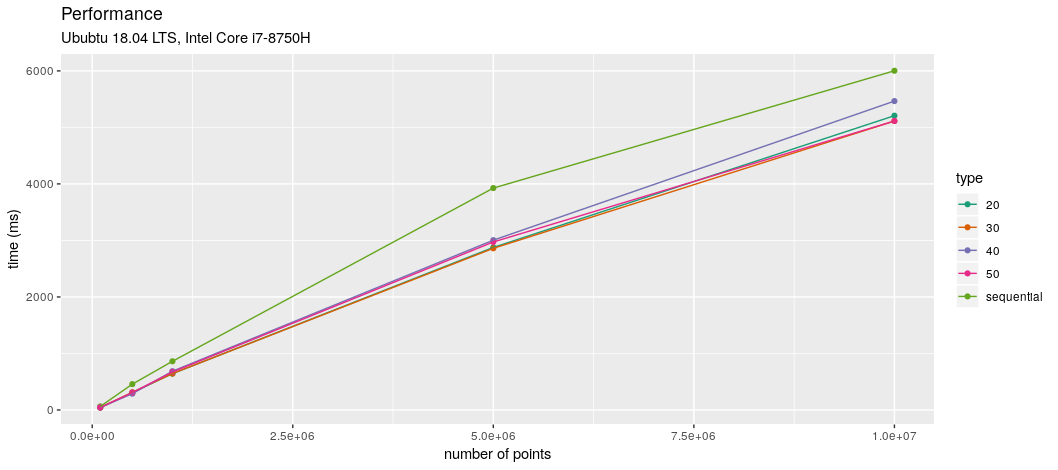
\includegraphics[width=0.4\textwidth,height=0.2\textheight]{performance}
		\caption{Performance data}
		\label{fig:performance}
	\end{figure}

\section{Conclusion}
\label{sec:coclusion}

	We`ve considered in details the process of designing and implementing the UAEM as well unified data structures for it. In this model a generic interface of a ``divide-and-conquer'' algorithm was created. This allows us to execute the algorithms which are implemented according to this model both sequentially and in parallel. Apart from that concatenable queue was implemented and served as the basis for the model described above.

	Using the data structure allowed to significantly reduce the time and computational resources for solving set of problems, such as constructing the convex hull. The algorithmic environment was implemented in Java programming language using its standard library. The main advantages of the developed algorithm are optimized preprocessing stage and the efficiently implemented merge step, due to the usage of concatenable queue.

	The performance comparison for both types of execution allows to conclude that the algorithm has high level of parallelism. We`ve achieved speedup of $28\%$ in the best case. It is easy to extend functionality of the created environment either by adding new or modifying existing algorithms. This flexibility is achieved by using the modular principle in its design and choosing optimal abstractions to represent algorithms.

\bibliographystyle{ACM-Reference-Format}
\bibliography{article-spaa20}

\end{document}
\endinput
